 \documentclass{beamer}
  %\usepackage[utf8]{inputenc}
  \usepackage{fontspec}  %pour xelatex
 \usepackage{xunicode}  %pour xelatex
  \usetheme{Montpellier}
   \usepackage{color}
   \usepackage{xcolor}
   \usepackage{graphicx}
   \usepackage{ulem}
%   \usepackage{xkeyval}
   \usepackage{pst-tree}
   \usepackage{tabularx}
   \usepackage[french]{babel}
 %  \usepackage{pstcol,pst-fill,pst-grad}
  \setbeamercolor{normal text}{fg=black}
 \setbeamercolor{section in head/foot}{fg=black}
  \setbeamercolor{subsection in head/foot}{fg=blue}
\beamerboxesdeclarecolorscheme{blocbleu}{black!60!white}{black!20!white}
\beamerboxesdeclarecolorscheme{blocimage}{black!60!white}{black!10!white}
\setbeamercolor{section in toc}{fg=black}
\setbeamercolor{subsection in toc}{fg=blue}
\date{}
%\usepackage{titlesec}
\usepackage{soul}


\AtBeginSection[]
{
 \begin{frame}
  \tableofcontents[currentsection,hideallsubsections]
 \end{frame}
}

\AtBeginSubsection[]
{
  \begin{frame}
  \tableofcontents[currentsection,currentsubsection]
  \end{frame}
}
  \title{{\textcolor{red}{Chapitre 2 - Les échanges de marchandises}}}

\usepackage{ifthen}
\makeatletter
\renewcommand\section{\@startsection
{section}{1}{0mm}
{\baselineskip}
{0.5\baselineskip}
{\normalfont\normalsize\textbf}}
\makeatother


\begin{document}

\newboolean{Professeur}
\setboolean{Professeur}{true} % « true» (vrai) si le document est le document du professeur (sans trous). « Professeur » a la valeur « false » par défaut. Il faut donc décommenter la ligne pour mettre « Professeur » à « true »
\newcommand{\Trouer}[1]{
\ifthenelse{\boolean{Professeur}} % si « Professeur » est vrai,
{\textbf{#1}} %les mots cachés sont en gras
{\underline{\phantom{#1.5}}} % (else) sinon les mots sont remplacés par une ligne sur laquelle l'élève peut écrire.
}

\newcommand{\df}[2]{\textcolor{red}{\underline{#1}: #2}}

\newcommand{\doc}[1]{
\begin{flushright}
\fbox{Documents : #1}
\end{flushright}
}

\newcommand{\con}[1]{\textcolor{blue}{\underline{Consigne}: #1}}

\newcommand{\rep}[1]{\textcolor{green}{\underline{Réponse}: #1}}

\begin{frame}
 \titlepage %{CHAPITRE 2 - LES IDENTIT�S MULTIPLES DE LA PERSONNE}
 \end{frame}
 \begin{frame}
Fil directeur : comprendre par quels lieux et par quels moyens de transports se déplace un produit.
 \end{frame}

\section{I/ Etude de cas : le trajet de l'ipod.}

\begin{frame}

\doc{4 p. 193}

\con{A partir de la carte, décrit le trajet de l'ipod de sa conception à sa vente.}

\rep{Méthode de lecture de carte.}
\end{frame}

\begin{frame}
\doc{bout de video sur usine de Foxconn}

\con{décrit les conditions de vie et de travail des ouvriers chinois.}

\end{frame}

\begin{frame}
Depuis 1945, les \Trouer{échanges} augmentent de plus en plus. Notre mode de vie est basé sur des produits fabriqués et transportés depuis \Trouer{l'autre bout du monde}. Au coeur de ces échanges se situent les \Trouer{grandes entreprises internationales} qui gèrent les transports maritimes par conteneurs. \\

Chiffres à connaître : 
80\% des échanges mondiaux transitent par la voie maritime \\
les portes-conteneurs transportent les 2/3 des marchandises dans le monde.

\end{frame}

\section{II/ Les pôles et flux majeurs des échanges mondiaux.}

-> croquis : doit mettre TITRE / LEGENDE / ECHELLE / ORIENTATION
-> tout mettre sur la carte. Elève doit retrouver à quoi ça correspond + hiérarchiser la légende.
-> localiser et situer qq gds points de passages stratégiques (canaux et détroits)

\begin{frame}
\includegraphics[width=10cm]{echanges-mondiaux.eps}
\end{frame}

  \end{document}